% संपूर्ण मराठी ग्रंथातील प्रकरण 5: अंकगणितीकरण
% हा संपादनयोग्य स्रोतखंड आहे. संकलनासाठी संपूर्ण स्रोतसंग्रहातील
% अक्षररूपे, पूर्वभाग, चिन्हव्याख्या आणि आकृती-स्रोत आवश्यक आहेत.
% मूळ: Open Logic Project; मजकूर आणि रूपांतर CC BY 4.0.
% यंत्रानुवाद, दुरुस्ती आणि तपासणी: OpenAI Codex —
% GPT-5.6 Sol आणि GPT-6 Sol, दोन्ही Ultra effort.
% दुरुस्ती-पुनरावलोकन: GPT-6.1 Sol, Ultra effort.
\chapter{अंकगणितीकरण}\label{sfr:arith::chap}
\begin{editorial}
या प्रकरणातील सामग्री अनौपचारिक संचसिद्धान्तात संख्याप्रणालींची रचना
मांडते. ती टिम बटन यांच्या Open Set Theory या ग्रंथातून घेतली आहे.
\end{editorial}






\section{$\Nat$ पासून $\Int$ कडे}\label{sfr:arith:int:sec}

येथे दोन मूलभूत निरीक्षणे आहेत:
	\begin{enumerate}
		\item प्रत्येक पूर्णांक $n - m$ या रूपात लिहिता येतो, जेथे $n, m \in\Nat$.
		\item $n - m$ या व्यंजकात सांकेतिक केलेली माहिती $\tuple{n, m}$ या क्रमित जोडीद्वारेही तितकीच सांकेतिक करता येते.
	\end{enumerate}
नैसर्गिक संख्यांच्या क्रमित जोड्या $\Nat^2$ चे घटक आहेत हे आपल्याला आधीच माहीत आहे. आणि आपण $\Nat$ समजतो असे गृहीत धरत आहोत. त्यामुळे या दोन निरीक्षणांवर आधारलेली एक भोळी सूचना पुढे करता येईल: \emph{नैसर्गिक संख्यांच्या क्रमित जोड्यांना पूर्णांक म्हणून हाताळू या}.

प्रत्यक्षात ही सूचना अतिशय भोळी आहे. अर्थात, $0- 2 = 4 - 6$ असले पाहिजे असे आपल्याला हवे आहे. पण स्पष्टपणे $\tuple{0, 2 }\neq \tuple{4, 6}$. त्यामुळे $\Nat^2$ हाच पूर्णांकांचा संच आहे असे सरळ म्हणता येत नाही.

मागील अडचणीचे सामान्यीकरण केल्यास आपल्याला पुढील अट हवी आहे:
	$$a - b = c - d \text{ तेव्हा आणि केवळ तेव्हाच }a + d = c + b$$
(पूर्णांकांचे वर्तन \emph{असेच अभिप्रेत} आहे हे स्पष्ट असावे: दोन्ही बाजूंना फक्त $b$ आणि $d$ मिळवा.) हे वर्तन निश्चित करण्याचा सोपा मार्ग म्हणजे क्रमित जोड्यांमधील $\Intequiv$ हा तुल्यता संबंध पुढीलप्रमाणे व्याख्यायित करणे:
$$\tuple{ a, b } \Intequiv \tuple{c, d}\text{ तेव्हा आणि केवळ तेव्हाच }a + d = c + b$$
आता हा तुल्यता संबंध आहे हे दाखवावे लागेल.
\begin{prop} $\Intequiv$ हा तुल्यता संबंध आहे.
\end{prop}
	\begin{proof}
	$\Intequiv$ परावर्ती, सममित आणि संक्रमक आहे हे दाखवले पाहिजे.

	\emph{परावर्तिता:} $a + b = b + a$ असल्यामुळे स्पष्टपणे $\tuple{a, b} \Intequiv \tuple{a, b}$.

	\emph{सममितता:} $\tuple{a, b} \Intequiv \tuple{c, d}$ असे समजा; म्हणजे $a + d = c + b$. मग $c + b = a + d$, त्यामुळे $\tuple{c, d} \Intequiv \tuple{a, b}$.

	\emph{संक्रमकता:} $\tuple{a, b} \Intequiv \tuple{c, d}\Intequiv \tuple{m, n}$ असे समजा. त्यामुळे $a + d = c + b$ आणि $c + n = m + d$. म्हणून $a + d + c + n = c + b + m + d$, व म्हणून $a + n = m + b$. परिणामी $\tuple{a, b } \Intequiv \tuple{m, n}$.
\end{proof}

आता या तुल्यता संबंधाचा वापर करून तुल्यतावर्ग घेता येतात:

\begin{defn}
		नैसर्गिक संख्यांच्या क्रमित जोड्यांचे $\Intequiv$ अंतर्गत तुल्यतावर्ग म्हणजे पूर्णांक; म्हणजेच $\Int = \equivclass{\Nat^2}{\Intequiv}$.
\end{defn}

या संकेतजनक व्याख्येबद्दल अनेक निरनिराळ्या \emph{तात्त्विक} प्रतिक्रिया असू शकतात. त्या प्रतिक्रियांचा विचार करण्यापूर्वी मात्र काही तांत्रिक तपशील पुढे नेणे उपयुक्त ठरेल.

पूर्णांक म्हणजे काय हे ठरवल्यावर त्यांच्यावरील मूलभूत फलने आणि संबंध व्याख्यायित करावे लागतील. ज्या $\Intequiv$ अंतर्गत तुल्यतावर्गात $\tuple{m, n}$ हा घटक आहे, त्या वर्गासाठी $\equivrep{m, n}{\Intequiv}$ असे लिहू या.\footnote{टीप: \ref{sfr:rel:eqv:def:equivalenceclass} मध्ये दिलेले संकेतन वापरल्यास त्याच वर्गासाठी आपण $\equivrep{\tuple{m,n}}{\Intequiv}$ असे लिहिले असते. पण ते वाचायला जरा कठीण आहे.} म्हणजे:
	$$\equivrep{m, n}{\Intequiv} = \Setabs{\tuple{a, b} \in \Nat^2}{\tuple{a, b}\Intequiv \tuple{m, n}}$$
आता काही व्याख्या देऊ:
	\begin{align*}
		\equivrep{a, b}{\Intequiv} + \equivrep{c, d}{\Intequiv} &= \equivrep{a + c, b + d}{\Intequiv}\\
		\equivrep{a, b}{\Intequiv} \times \equivrep{c, d}{\Intequiv} &= \equivrep{a c + b  d, a  d + b c}{\Intequiv}\\
		\equivrep{a, b}{\Intequiv} \leq \equivrep{c, d}{\Intequiv} &\text{ तेव्हा आणि केवळ तेव्हाच }a + d \leq b + c
	\end{align*}
(प्रथेप्रमाणे, स्वयंसिद्धे वाचायला सोपी व्हावीत म्हणून मी `$(a \times b)$' या अर्थी `$ab$' लिहित आहे.) आता या व्याख्या \emph{अपेक्षेप्रमाणे} वागतात याची खात्री केली पाहिजे. याचा नेमका अर्थ उलगडून संपूर्ण पडताळणी करणे बरेच कष्टाचे आहे; तपशील आपण \ref{sfr:arith:check:sec} कडे सोपवतो. पण थोडक्यात: सर्व काही व्यवस्थित चालते!

आता फक्त एक गोष्ट उरते. आपण नैसर्गिक संख्यांच्या साहाय्याने
पूर्णांकांची रचना केली आहे. पण त्यामुळे नैसर्गिक संख्या \emph{स्वतः
पूर्णांक नसतील}. याचे तात्त्विक महत्त्व आपण \ref{sfr:arith:ref:sec} मध्ये
पुन्हा पाहू. मात्र पूर्णपणे तांत्रिक दृष्टीने, नैसर्गिक संख्यांना
पूर्णांक \emph{म्हणून} हाताळण्याची काही पद्धत आपल्याला हवी. कल्पना अगदी
सोपी आहे: प्रत्येक $n \in \Nat$ साठी $n_\Int = \equivrep{n, 0}{\Intequiv}$
असे आपण ठरवतो. ही व्याख्या सुयोग्य रीतीने वागते याची, म्हणजे कोणत्याही
$m, n \in \Nat$ साठी पुढील अटी पूर्ण होतात याची खात्री केली पाहिजे:
\begin{align*}
	(m + n)_\Int &= m_\Int + n_\Int\\
	(m \times n)_\Int &= m_\Int \times n_\Int\\
	m \leq n &\liff m_\Int \leq n_\Int
\end{align*}
ही सर्व पडताळणी अगदी सरळ आहे. उदाहरणार्थ, दुसरी अट खरी आहे हे
दाखवताना नैसर्गिक संख्यांच्या परिचित वर्तनाचा थेट वापर करून पुढीलप्रमाणे
युक्तिवाद करता येतो:
	\begin{align*}
		(m \times n)_\Int  &= \equivrep{m \times n, 0}{\Intequiv} \\
		&= \equivrep{m \times n + 0 \times 0, m \times 0 + 0 \times n}{\Intequiv} \\
		&= \equivrep{m, 0}{\Intequiv} \times \equivrep{n, 0}{\Intequiv} \\
		&= m_\Int \times n_\Int
	\end{align*}
इतर दोन अटी पडताळण्याचे काम सरावासाठी सोडतो.
\begin{prob}
	कोणत्याही $m, n \in \Nat$ साठी $(m + n)_\Int = m_\Int + n_\Int$ आणि $m \leq n \liff m_\Int \leq n_\Int$ हे दाखवा.
\end{prob}







\section{$\Int$ पासून $\Rat$ कडे}\label{sfr:arith:rat:sec}

अनौपचारिक संचसिद्धान्त वापरून नैसर्गिक संख्यांपासून पूर्णांकांची रचना कशी
करायची हे आपण नुकतेच पाहिले. आता अगदी त्याच प्रकारे पूर्णांकांपासून
परिमेय संख्यांची रचना कशी करायची ते पाहू. सुरुवातीची निरीक्षणे अशी:
\begin{enumerate}
	\item प्रत्येक परिमेय संख्या $\nicefrac{i}{j}$ या रूपात लिहिता येते,
	जेथे $i$ आणि $j$ दोन्ही पूर्णांक असतात, पण $j$ शून्येतर असतो.
	\item $\nicefrac{i}{j}$ या व्यंजकात सांकेतिक केलेली माहिती
	$\tuple{ i, j}$ या क्रमित जोडीद्वारेही तितकीच सांकेतिक करता येते.
\end{enumerate}
यावरून परिमेय संख्यांकडे $\Int \times (\Int \setminus \{0_\Int\})$
मधून घेतलेल्या क्रमित जोड्या \emph{म्हणून} पाहणे हा स्वाभाविक मार्ग
वाटेल. मात्र आधीप्रमाणे ही कल्पना जरा अतिभोळी ठरेल, कारण आपल्याला
$\nicefrac{3}{2} = \nicefrac{6}{4}$ हवे आहे, पण $\tuple{ 3, 2}\neq \tuple{ 6,
4}$. अधिक सर्वसाधारणपणे आपल्याला पुढील अट हवी:
\[	\nicefrac{a}{b} = \nicefrac{c}{d} \text{ तेव्हा आणि केवळ तेव्हाच } a \times d = b \times c
\]
ही अट मिळवण्यासाठी $\Int \times (\Int \setminus \{0_\Int\})$ वरील
{तुल्यता संबंध} आपण पुढीलप्रमाणे व्याख्यायित करतो:
\[	\tuple{ a, b }\Ratequiv \tuple{ c, d} \text{ तेव्हा आणि केवळ तेव्हाच }a \times d = b \times c
\]
हा तुल्यता संबंध आहे हे तपासले पाहिजे. ही तपासणी बरीचशी $\Intequiv$
च्या प्रकरणासारखीच आहे आणि ती आपण सरावासाठी सोडू.
\begin{prob}
$\Ratequiv$ हा तुल्यता संबंध आहे हे दाखवा.
\end{prob}
त्यामुळे पुढील व्याख्या देता येते:
\begin{defn}
दुसरा घटक शून्येतर असलेल्या पूर्णांकांच्या जोड्यांचे $\Ratequiv$ अंतर्गत
तुल्यतावर्ग म्हणजे परिमेय संख्या. म्हणजेच $\Rat =
\equivclass{(\Int \times (\Int\setminus \{0_\Int\}))}{\Ratequiv}$.
\end{defn}

पूर्णांकांप्रमाणे येथेही काही मूलभूत क्रिया व्याख्यायित करायच्या आहेत.
$\tuple{i, j}$ हा घटक असलेला $\Ratequiv$ अंतर्गत तुल्यतावर्ग
$\equivrep{i,j}{\Ratequiv}$ असेल, तर आपण पुढील व्याख्या करतो:
\begin{align*}
	\equivrep{a, b}{\Ratequiv} + \equivrep{c, d}{\Ratequiv} &= \equivrep{ad + bc,  bd}{\Ratequiv}\\
	\equivrep{a, b}{\Ratequiv} \times \equivrep{c, d}{\Ratequiv} &= \equivrep{a  c, b d}{\Ratequiv}.
\intertext{या परिमेय संख्यांवर $r \leq s$ ची व्याख्या करण्यासाठी आपण पुढील तथ्य वापरतो: $r \le s$ तेव्हा आणि केवळ तेव्हाच $s - r$ हा फरक ऋण नसतो; म्हणजे $s - r$ हा $\nicefrac{i}{j}$ या रूपात लिहिता येतो, जेथे $i$ ऋणेतर आणि $j$~धन असतो:}
	\equivrep{a, b}{\Ratequiv} \leq \equivrep{c, d}{\Ratequiv} &\text{ तेव्हा आणि केवळ तेव्हाच }
	\equivrep{c, d}{\Ratequiv} - \equivrep{a, b}{\Ratequiv} =
	\equivrep{i_\Int, j_\Int}{\Ratequiv}
\end{align*}
\begin{quote}\small\textbf{स्रोतदुरुस्ती.} MRARITH-001: गोठवलेल्या इंग्रजी स्पष्टीकरणात “s-r is not negative” नंतर चुकून r-s ला ऋणेतर अपूर्णांकाच्या रूपात लिहिले आहे. लगेचची प्रदर्शित व्याख्या पुन्हा s-r वापरते. मराठी मजकुरात या दोन्ही नियंत्रक ठिकाणांशी सुसंगत s-r वापरले आहे.\end{quote}
असे काही $i \in \Nat$ आणि $0 \neq j \in \Nat$ असले पाहिजेत.

त्यानंतर या व्याख्या \emph{अपेक्षेप्रमाणे} वागतात हे तपासावे लागेल;
ही तपासणी आपण \ref{sfr:arith:check:sec} कडे सोपवतो. आणि त्या खरोखर तशाच
वागतात!{} शेवटी, पूर्णांकांना परिमेय संख्या \emph{म्हणून} हाताळण्याची
काही पद्धत हवी; म्हणून प्रत्येक $i \in \Int$ साठी $i_\Rat =
\equivrep{i, 1_\Int}{\Ratequiv}$ असे आपण ठरवतो. हे सर्व सुयोग्य रीतीने
वागते याची तपासणीही आपण \ref{sfr:arith:check:sec} मध्ये करतो.

\begin{prob}
कोणत्याही $i, j \in \Int$ साठी $(i + j)_\Rat = i_\Rat+ j_\Rat$ आणि $(i \times j)_\Rat =
i_\Rat \times j_\Rat$ आणि $i \leq j \liff i_\Rat \leq j_\Rat$ हे दाखवा.
\end{prob}








\section{वास्तव संख्या-रेषा}\label{sfr:arith:real:sec}

पुढील पायरी म्हणजे परिमेय संख्यांपासून वास्तव संख्यांची रचना कशी करायची
हे दाखवणे. त्याआधी वास्तव संख्यांचे \emph{वैशिष्ट्य} नेमके काय आहे हे
समजून घ्यावे लागेल.

वास्तव संख्या परिमेय संख्यांसारख्याच बऱ्याच अंशी वागतात. (तांत्रिक
भाषेत, दोन्ही \emph{क्रमित क्षेत्रांची} उदाहरणे आहेत; त्याची व्याख्या
\ref{sfr:arith:check:orderedfield} मध्ये पाहा.) आता, तुम्ही \ref{sfr:siz::chap}
मधील सराव सोडवले असतील, तर वास्तव संख्या परिमेय संख्यांपेक्षा काटेकोरपणे
अधिक आहेत, म्हणजे $\cardless{\Rat}{\Real}$, हे तुम्हाला माहीत असेल.
हे कँटर यांनी प्रथम सिद्ध केले. परंतु अपरिमेय संख्या, म्हणजे परिमेय
नसलेल्या वास्तव संख्या, अस्तित्वात आहेत हे सुमारे अडीच सहस्रकांपासून
माहीत आहे. खरे तर:
\begin{quote}\small\textbf{स्रोतदुरुस्ती.} MRARITH-002: गोठवलेल्या इंग्रजीतील निष्क्रिय केलेली तळटीप \ensuremath{\sqrt{2}} हे धन आणि ऋण अशी दोन्ही मुळे दर्शवते असे म्हणते. पारंपरिक मूलचिन्ह मात्र मुख्य, ऋणेतर वर्गमूळ दर्शवते; म्हणून मराठीतील निष्क्रिय तळटीप दुरुस्त केली आहे. सक्रिय वाचनीय मजकुरावर याचा परिणाम नाही.\end{quote}
\begin{thm}\label{sfr:arith:real:root2irrational}
$\sqrt{2}$ ही परिमेय संख्या नाही; म्हणजे $\sqrt{2} \notin \Rat$.
\end{thm}

\begin{proof}
व्याघातासाठी $\sqrt{2}$ ही परिमेय संख्या आहे असे समजा. मग काही नैसर्गिक
संख्या $m$ आणि $n$ यांसाठी $\sqrt{2} = \nicefrac{m}{n}$. हा अपूर्णांक
यापुढे संक्षिप्त करता येणार नाही अशा रीतीने आपण $m$ आणि $n$ निवडू शकतो.
पुनर्मांडणी केल्यास $m^{2} = 2n^{2}$. येथून सिद्धता दोन प्रकारे पूर्ण
करता येते:

\emph{प्रथम, भूमितीय रीतीने} (टेनेनबाउम यांच्या पद्धतीने).\footnote{ही
सिद्धता Conway (2006) यांनी नोंदवली आहे.} पुढील चौरस पाहा:
\begin{center}
	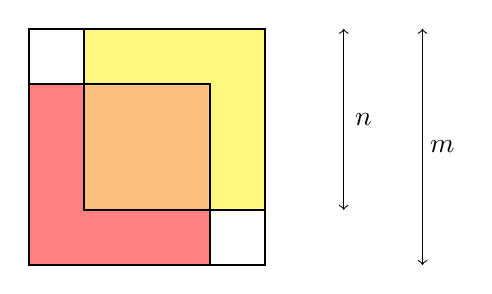
\begin{tikzpicture}
		\draw[thick] (0,0) rectangle (3,3);
		\draw[thick, fill=red!50] (0,0) rectangle (2.3,2.3);
		\draw[thick, fill=yellow!50] (0.7,0.7) rectangle (3, 3);
		\draw[thick, fill=orange!50] (0.7,0.7) rectangle (2.3, 2.3);
		\draw[<->] (4, 0.7)--(4, 3);
		\node at (4.25, 1.85) (n) {$n$};
		\draw[<->] (5, 0)--(5, 3);
		\node at (5.25, 1.5) (m) {$m$};
	\end{tikzpicture}
\end{center}
$m^2 = 2n^2$ असल्यामुळे $n$ बाजू असलेले दोन चौरस ज्या प्रदेशात
एकमेकांवर येतात त्याचे क्षेत्रफळ, या दोन्ही चौरसांपैकी एकानेही न झाकलेल्या
प्रदेशाच्या क्षेत्रफळाइतके आहे; म्हणजे नारिंगी चौरसाचे क्षेत्रफळ हे दोन
न रंगवलेल्या चौरसांच्या क्षेत्रफळांच्या बेरजेइतके आहे. नारिंगी चौरसाची
बाजू $p$ आणि प्रत्येक न रंगवलेल्या चौरसाची बाजू $q$ असेल, तर $p^2 =
2q^2$. पण आता $p < m$, $q < n$ आणि $p, q \in \Nat$ असून
$\sqrt{2} = \nicefrac{p}{q}$. हे $m$ आणि $n$ शक्य तितके लहान निवडले
होते या तथ्याशी विसंगत आहे.

\emph{दुसरी, आकारिक रीतीने.} $m^{2} = 2n^{2}$ असल्यामुळे $m$ सम आहे.
($x$ विषम असेल, तर $x^2$ विषम असतो हे सहज दाखवता येते.) म्हणून काही
$r \in \Nat$ साठी $m = 2r$. पुनर्मांडणी केल्यास $2r^2 = n^2$,
त्यामुळे $n$ देखील सम आहे. म्हणून $m$ आणि $n$ दोन्ही सम आहेत, आणि
त्यामुळे $\nicefrac{m}{n}$ हा अपूर्णांक पुढे \emph{संक्षिप्त करता येतो}.
व्याघात!
\end{proof}

जाताजाता, या आकृतीवरील सिद्धतेमुळे पर्यायी विभाग
मधील सामग्रीचा पुन्हा विचार करता येतो. टेनेनबाउम (1927--2005) हे पूर्णपणे
आधुनिक गणितज्ञ होते; तरी ही सिद्धता निर्विवादपणे सुंदर, पूर्णतः तर्कशुद्ध
आहे आणि भूमितीय अंतःप्रज्ञेला आवाहन करते!
\begin{quote}\small\textbf{स्रोतदुरुस्ती.} MRARITH-003: गोठवलेल्या इंग्रजी मजकुरात निधनवर्ष 2006 दिले आहे. टेनेनबाउम यांच्या स्मृतिस्थळावरील चरित्र नोंद निधनाची तारीख 4 मे 2005 देते; मराठी मजकुरात 1927--2005 वापरले आहे.\end{quote}

कसेही असो, वास्तव संख्या परिमेय संख्यांपेक्षा ``अधिक विस्तृत'' आहेत.
एका अर्थाने परिमेय संख्यांमध्ये ``पोकळ्या'' आहेत आणि वास्तव संख्या त्या
भरून काढतात. वायश्ट्रास यांच्या लक्षात आले की या वर्णनातून वास्तव
संख्यांचा एकच गुणधर्म व्यक्त होतो, जो त्यांना परिमेय संख्यांपासून वेगळे
करतो; तो म्हणजे संपूर्णता गुणधर्म: \emph{ऊर्ध्वबंध असलेल्या वास्तव
संख्यांच्या प्रत्येक अरिक्त संचाला लघुतम ऊर्ध्वबंध असतो.}

परिमेय संख्यांना संपूर्णता गुणधर्म नाही हे सहज दिसते. उदाहरणार्थ,
$\sqrt{2}$ पेक्षा लहान परिमेय संख्यांचा पुढील संच पाहा:
\[	\Setabs{p \in \Rat}{p^2 < 2 \text{ किंवा }p < 0}
\]
या संचाला परिमेय संख्यांमध्ये ऊर्ध्वबंध आहे; उदाहरणार्थ, त्याचे सर्व
घटक< $3$ पेक्षा लहान आहेत. पण त्याचा लघुतम ऊर्ध्वबंध कोणता?
आपल्याला ` $\sqrt{2}$ ' असे म्हणायचे आहे; पण $\sqrt{2}$ ही \emph{परिमेय
संख्या नाही} हे आपण नुकतेच पाहिले. आणि $\sqrt{2}$ पेक्षा मोठी अशी कोणतीही
\emph{लघुतम} परिमेय संख्या नाही. म्हणून या संचाला ऊर्ध्वबंध आहे, पण लघुतम
ऊर्ध्वबंध नाही. त्यामुळे परिमेय संख्यांमध्ये संपूर्णता गुणधर्माचा अभाव आहे.

याउलट, सांतत्याला संपूर्णता गुणधर्म स्वभावतः असायला हवा. $\sqrt{2}$ ही
केवळ वास्तव संख्या असावी एवढेच आपल्याला नको; परिमेय संख्या-रेषेतील सर्व
``पोकळ्या'' भरायच्या आहेत. खरे तर सांतत्यात स्वतःमध्येच कोणतीही ``पोकळी''
नसावी असे आपल्याला हवे आहे. संपूर्णतेद्वारे नेमके हेच मिळेल.







\section{$\Rat$ पासून $\Real$ कडे}\label{sfr:arith:cuts:sec}

मूलतः, संपूर्णता गुणधर्म असे दाखवतो की वास्तव संख्या-रेषेवरील कोणताही
$\alpha$ बिंदू त्या रेषेचे अचूक दोन भाग करतो: खालच्या भागाचा $\alpha$
हा लघुतम ऊर्ध्वबंध असतो आणि वरच्या भागाचा $\alpha$ हा महत्तम निम्नबंध
असतो. परिमेय संख्यांपासून वास्तव संख्यांची \emph{रचना} करण्यासाठी
डेडेकिंड यांनी वास्तव संख्यांना परिमेय संख्यांचे विभाजन करणारे
\emph{छेद} मानण्याची सूचना केली. म्हणजेच, $< \sqrt{2}$ असलेल्या परिमेय
संख्यांना $> \sqrt{2}$ असलेल्या परिमेय संख्यांपासून वेगळे करणाऱ्या
\emph{छेदाशी} आपण $\sqrt{2}$ ची एकरूपता मानतो.

ही मांडणी नीट नेमकी करू या. परिमेय संख्यांचे दोन भाग केले, तर आपण केलेले
विभाजन केवळ त्याचा \emph{खालचा} भाग विचारात घेऊन अनन्यपणे ओळखता येते.
म्हणून नेमकी पुढील व्याख्या देऊ:

\begin{defn}[छेद]
\emph{छेद} $\alpha$ म्हणजे परिमेय संख्यांचा असा कोणताही अरिक्त उचित
आरंभीचा खंड ज्याला महत्तम घटक नाही. म्हणजे $\alpha$ हा छेद तेव्हा आणि
केवळ तेव्हाच असतो, जेव्हा:
\begin{enumerate}
	\item \emph{अरिक्त, उचित}: $\emptyset \neq \alpha \subsetneq \Rat$
	\item \emph{आरंभीचा}: सर्व $p,q \in \Rat$ साठी: $p < q \in \alpha$ असेल, तर $p \in \alpha$
	\item \emph{महत्तम घटक नाही}: प्रत्येक $p \in \alpha$ साठी $p < q$ असे काही $q \in \alpha$ असते
\end{enumerate}
मग $\Real$ हा छेदांचा संच आहे.
\end{defn}

आता $\sqrt{2} = \Setabs{p \in \Rat}{p^2 < 2\text{
किंवा }p < 0}$ असे म्हणता येते. अर्थात, हा खरोखर \emph{छेद} आहे हे
तपासले पाहिजे; ती तपासणी आपण \ref{sfr:arith:check:sec} कडे सोपवतो.

आधीप्रमाणेच, काही वस्तूंची व्याख्या केल्यानंतर त्यांच्यावरील मूलभूत
फलने आणि संबंध व्याख्यायित करावे लागतात. एका सोप्या व्याख्येपासून सुरुवात करू:
\begin{align*}
	\alpha \leq \beta \text{ तेव्हा आणि केवळ तेव्हाच }\alpha \subseteq \beta
\end{align*}
क्रमाची ही व्याख्या छेदांच्या संचाला संपूर्णता गुणधर्म आहे हा मध्यवर्ती
निष्कर्ष \emph{मांडू} देते. पूर्णपणे उलगडल्यास विधानाचे रूप असे आहे.
$S$ हा ऊर्ध्वबंध असलेला छेदांचा अरिक्त संच असेल, तर $S$ ला लघुतम
ऊर्ध्वबंध असतो. अधिक तपशीलाने: $S$ चा ऊर्ध्वबंध असणारा $\lambda$ हा छेद
असतो, म्हणजे $(\forall \alpha \in S)\alpha \subseteq \lambda$, आणि
$\lambda$ हा अशा छेदांपैकी लघुतम असतो, म्हणजे $(\forall \beta \in \Real)((\forall \alpha \in S)\alpha \subseteq \beta \lif \lambda \subseteq \beta)$. आता या निष्कर्षाची सिद्धता पाहा:

\begin{thm}\label{sfr:arith:cuts:realcompleteness}
छेदांच्या संचाला संपूर्णता गुणधर्म आहे.
\end{thm}

\begin{proof}
$S$ हा ऊर्ध्वबंध असलेला छेदांचा कोणताही अरिक्त संच असू द्या. $\lambda
= \bigcup S$ असे ठरवू.
प्रथम $\lambda$ हा छेद आहे असा दावा करू:
\begin{enumerate}
\item $S$ अरिक्त असल्यामुळे $S$ मध्ये किमान एक छेद आहे, म्हणून
$\emptyset \neq \lambda$. $S$ हा छेदांचा संच असल्यामुळे $\lambda
\subseteq \Rat$. $S$ ला ऊर्ध्वबंध असल्यामुळे प्रत्येक $\alpha \in S$
मधून अनुपस्थित असलेली अशी काही $p \in \Rat$ आहे. म्हणून $p\notin \lambda$,
आणि परिणामी $\lambda \subsetneq \Rat$.
\begin{quote}\small\textbf{स्रोतदुरुस्ती.} MRARITH-004: गोठवलेल्या इंग्रजी सिद्धतेत \ensuremath{\lambda} अरिक्त असल्याचे पहिले कारण चुकून “S has an upper bound” असे दिले आहे. आवश्यक आणि आधीच गृहीत असलेले कारण S अरिक्त असणे हे आहे; मराठी सिद्धतेत तेच वापरले आहे. पुढील उचित-उपसंच युक्तिवादासाठी मात्र ऊर्ध्वबंधाचे गृहीतक योग्य आहे.\end{quote}
\item $p < q \in \lambda$ असे समजा. मग $q \in \alpha$ असे काही
$\alpha \in S$ आहे. $\alpha$ हा छेद असल्यामुळे $p \in \alpha$.
म्हणून $p \in \lambda$.
\item $p \in \lambda$ असे समजा. मग $p \in \alpha$ असे काही
$\alpha \in S$ आहे. $\alpha$ हा छेद असल्यामुळे $p < q$ असे काही
$q \in \alpha$ आहे. म्हणून $q \in \lambda$.
\end{enumerate}
यावरून दावा सिद्ध होतो. शिवाय, स्पष्टपणे $(\forall \alpha \in S)\alpha
\subseteq \bigcup S = \lambda$, म्हणजे $\lambda$ हा $S$ चा ऊर्ध्वबंध
आहे. आता $\beta \in \mathbb{R}$ हाही ऊर्ध्वबंध आहे असे समजा, म्हणजे
$(\forall \alpha \in S)\alpha \subseteq \beta$. कोणत्याही $p \in \Rat$
साठी, $p \in \lambda$ असेल तर $p \in \alpha$ असे काही $\alpha \in S$
आहे, आणि त्यामुळे $p \in \beta$. सार्वत्रिकीकरण केल्यास $\lambda
\subseteq \beta$. म्हणून $\lambda$ हा $S$ चा \emph{लघुतम} ऊर्ध्वबंध आहे.
\end{proof}

म्हणून आपल्याकडे संपूर्णता गुणधर्म पूर्ण करणाऱ्या अनेक वस्तू आहेत.
हे सांगण्याचा एक मार्ग असा: आपल्या छेदांमध्ये ``पोकळ्या'' नाहीत.
(त्यामुळे परिमेय संख्यांऐवजी वास्तव संख्यांचे आणखी ``छेद'' घेतल्यास
काही रोचक नवी वस्तू मिळणार नाही.)

पुढे वास्तव संख्यांवरील काही क्रिया व्याख्यायित केल्या पाहिजेत. प्रत्येक
$p \in \Rat$ साठी $p_\Real = \Setabs{q \in \Rat}{q < p}$ असे ठरवून
परिमेय संख्यांना वास्तव संख्यांत अंतःस्थापित करण्यापासून सुरुवात करू.
मग पुढील व्याख्या करतो:
\begin{align*}
	\alpha + \beta &= \Setabs{p + q}{p \in \alpha \land q \in \beta}\\
	\alpha \times \beta &=
	\Setabs{p \times q}{0 \leq p \in \alpha \land 0 \leq q \in \beta} \cup 0_\Real & \text{जर }\alpha, \beta \geq 0_\Real
\end{align*}
\begin{quote}\small\textbf{स्रोतदुरुस्ती.} MRARITH-005: गोठवलेल्या इंग्रजी गुणाकार-व्याख्येत शून्याचा छेद एकदाच 0\textasciicircum{}R असा विसंगत ऊर्ध्वनिर्देशांक वापरून लिहिला आहे; त्याच परिच्छेदातील सर्व नियंत्रक संकेतन 0\_R वापरते. मराठी सूत्रात 0\_R वापरले आहे.\end{quote}
गुणाकाराची इतर प्रकरणे हाताळण्यासाठी प्रथम $0_\Real \times \alpha = 0_\Real = \alpha \times 0_\Real$ असे ठरवू आणि पुढील व्याख्या करू:
\begin{quote}\small\textbf{स्रोतदुरुस्ती.} MRARITH-006: गोठवलेल्या इंग्रजी स्रोताने शून्यासोबतच्या गुणाकाराची ही आवश्यक व्याख्या त्याच ओळीवर निष्क्रिय केली आहे; त्यामुळे एक घटक ऋण व दुसरा शून्य असलेली प्रकरणे पुढील प्रकरणनिहाय व्याख्येत येत नाहीत. स्रोताच्याच निष्क्रिय सूत्राला मराठीत सक्रिय केले आहे.\end{quote}
\begin{align*}
	-\alpha &= \Setabs{p - q}{p < 0 \land q \notin \alpha}
\end{align*}
आणि मग पुढीलप्रमाणे ठरवू:
\begin{align*}
	\alpha \times \beta &\defis
	\begin{cases}
		\mathord{-}\alpha \times \mathord{-}\beta &\text{जर }\alpha < 0_\Real\text{ आणि }\beta < 0_\Real\\
		\mathord{-}(\mathord{-}\alpha \times \beta) &\text{जर }\alpha < 0_\Real \text{ आणि }\beta > 0_\Real\\
		\mathord{-}(\alpha \times \mathord{-}\beta) &\text{जर }\alpha > 0_\Real \text{ आणि }\beta < 0_\Real
	\end{cases}
\end{align*}
यानंतर यांपैकी प्रत्येक व्याख्येतून नेहमी छेदच मिळतो हे तपासावे लागेल.
आणि शेवटी, अशा प्रकारे व्याख्यायित केलेले छेद अपेक्षेप्रमाणेच वागतात
हे दाखवणारी सोपी (पण लांबलचक) सिद्धता पूर्ण केली पाहिजे. मात्र हे सर्व
आपण \ref{sfr:arith:check:sec} कडे सोपवतो.







\section{काही तात्त्विक चिंतन}\label{sfr:arith:ref:sec}

तांत्रिक तपशील एवढेच. पण त्यातून साधले तरी काय?

एक तर, अगदी निर्विवादपणे, त्यातून आपल्याला काही {सुंदर} शुद्ध गणित
मिळाले. शिवाय काही खोल संकल्पनात्मक कामगिरीही झाली. वास्तव संख्या आणि
परिमेय संख्या यांतील निर्णायक फरक संपूर्णता गुणधर्म व्यक्त करतो, हे
ओळखणे ही एक सखोल अंतर्दृष्टी होती. तसेच, डेडेकिंड छेद म्हणून वास्तव
संख्यांची स्पष्ट रचना केल्यामुळे विश्लेषणाच्या विषयाला भक्कम आधार मिळतो.
छेदांपासून नेमके असेच क्षेत्र बनत असल्यामुळे \emph{संपूर्ण क्रमित क्षेत्र}
ही संकल्पना सुसंगत आहे, हे आपल्याला माहीत आहे.

एवढे असूनही, या कामगिरीबद्दलच्या काही शंका उघडपणे मांडल्या पाहिजेत.

पहिली शंका अशी की, वास्तव संख्यांचा परिचित (कदाचित अनंत) दशांश विस्तार
विचारात घेण्यापेक्षा छेदांच्या रूपात त्यांचा विचार करणे \emph{अधिक}
काटेकोर आहे, हे स्पष्ट नाही. दशांश विस्तारांनी वास्तव संख्यांची केलेली
ही ``रचना'' कोशी क्रमिकांद्वारे केलेल्या रचनेस काहीशी मिळतीजुळती आहे;
परंतु प्रत्यक्षात ती सतराव्या शतकाच्या प्रारंभापासूनच गणितज्ञांना मूलतः
माहीत होती (पाहा \ref{sfr:arith:cauchy:sec}). वास्तव संख्यांना संपूर्णता गुणधर्म
आहे याची जाणीव झाल्यामुळे काटेकोरपणात खरी वाढ झाली; वास्तव संख्यांची काही
विशिष्ट संच म्हणून रचना करता येणे हे कदाचित स्वतःपुरते फारसे रोचक नाही.

पूर्णांकांचे किंवा परिमेय संख्यांचे (त्याहून खूप सोपे) अंकगणितीकरण त्या
क्षेत्रांतील काटेकोरपणा वाढवते, हे तर आणखी कमी स्पष्ट आहे. येथे एक साधे
निरीक्षण उपयुक्त ठरेल. नैसर्गिक संख्यांच्या क्रमित जोड्यांचे तुल्यतावर्ग
म्हणून पूर्णांकांची \emph{रचना} केल्यानंतर, मग पूर्णांकांच्या क्रमित
जोड्यांचे तुल्यतावर्ग म्हणून परिमेय संख्यांची रचना केल्यानंतर, आणि मग
परिमेय संख्यांचे संच म्हणून वास्तव संख्यांची रचना केल्यानंतर आपण त्या
रचना लगेचच \emph{विसरून जातो}. विशेषतः, कोणालाही गणिती सिद्धतेत या
रचनांचा \emph{उपयोग} करावासा वाटणार नाही (त्या रचना अपेक्षेप्रमाणेच
वागतात हे सिद्ध करताना मात्र अर्थातच त्यांचा उपयोग करावा लागेल).
नैसर्गिक संख्यांच्या संचांच्या संचांच्या संचांच्या संचांच्या संचांच्या
संचांच्या एखाद्या संचाबद्दल बोलण्यापेक्षा वास्तव संख्येबद्दल थेट बोलणे
खूपच सोपे आहे.

या व्याख्या आपल्याला पूर्णांक, परिमेय संख्या किंवा वास्तव संख्या
\emph{नेमक्या काय आहेत}, \emph{सत्तामीमांसक दृष्ट्या सांगायचे तर}, हे
सांगतात, याबद्दल तर
सर्वाधिक शंका आहे. म्हणजे, वास्तव संख्या (उदाहरणार्थ) काही विशिष्ट संच
(संचांच्या संचांचे संच\ldots) \emph{आहेत}, हे संशयास्पद आहे. अशा
दृष्टिकोनासमोरील मुख्य अडथळा हा की ही रचना अनेक वेगवेगळ्या पद्धतींनी करता
आली असती. वास्तव संख्यांच्या बाबतीत खरोखर रोचक रीतीने भिन्न असलेल्या काही
रचना आहेत (पाहा \ref{sfr:arith:cauchy:sec}). पण काही वेगळ्या रचना मिळवण्याची
एक अगदी क्षुल्लक पद्धत अशी: \ref{sfr:rel:ref:sec} प्रमाणे आपण
क्रमित जोडीची व्याख्या किंचित वेगळी करू शकलो असतो; क्रमित जोडीची ही
पर्यायी संकल्पना वापरली असती, तर आपल्या रचना तितक्याच यशस्वी झाल्या
असत्या, पण शेवटी मिळालेल्या वस्तू वेगळ्या असत्या. त्यामुळे पूर्णांक,
परिमेय संख्या आणि वास्तव संख्या यांच्या अनेक प्रतिस्पर्धी संचसैद्धान्तिक
रचना आहेत. आता पूर्णांक (उदाहरणार्थ) \emph{त्या} संचांऐवजी \emph{हेच}
संच आहेत, असा दावा करणे केवळ मनमानीचे (आणि अडचणीचे) ठरेल.
(\ref{sfr:rel:ref:sec} प्रमाणे, Benacerraf (1965) यांनी
प्रसिद्ध केलेल्या युक्तिवादाचे हे एक उदाहरण आहे.)

आणखी एक मुद्दा उपस्थित करायला हवा: आपल्या रचनांमध्ये काहीतरी फारच
\emph{विचित्र} आहे. आपण नैसर्गिक संख्यांपासून सुरुवात केली. मग पूर्णांकांची
रचना केली आणि ``पूर्णांकांचा $0$'', म्हणजे $ \equivrep{0,0}{\Intequiv}$,
याची रचना केली. पण $0 \neq \equivrep{0,0}{\Intequiv}$. खरे तर, आपल्या
रचनांनुसार \emph{एकही} नैसर्गिक संख्या पूर्णांक नाही. पण हे सहजज्ञानाच्या
अगदी विरुद्ध वाटते. प्रत्यक्षात \ref{sfr:set:imp:sec} मध्ये आपण
फारसा युक्तिवाद न करता $\Nat \subseteq \Rat$ असा दावा केला होता. संख्या
नेमक्या \emph{काय आहेत} हे या रचना सांगत असतील, तर तो दावा उघडपणे असत्य
होता.

मग थोडे मागे हटून पाहिल्यास आपण कुठवर पोहोचलो? अनौपचारिक संचसिद्धान्तात
काम करताना आणि नैसर्गिक संख्या गृहीत धरताना, पूर्णांक, परिमेय संख्या आणि
वास्तव संख्या यांना काही विशिष्ट संच \emph{म्हणून वागवणे} आपल्याला शक्य
होते. त्या अर्थाने, या वस्तूंचे सिद्धान्त संचसिद्धान्तात
\emph{अंतःस्थापित} करता येतात. पण या अंतःस्थापनाचा तात्त्विक आशय अजिबात
सरळसोट नाही.

अर्थात, याने या विषयावरील शेवटचा शब्द सांगितलेला नाही!{} मुद्दा फक्त
एवढाच आहे. वास्तव संख्यांच्या अंकगणितीकरणाला खोल तात्त्विक महत्त्व
\emph{आहे} हे दाखवण्यासाठी आणखी काही \emph{तात्त्विक} युक्तिवाद आवश्यक असेल.









\section{क्रमित वलये आणि क्षेत्रे}\label{sfr:arith:check:sec}

या प्रकरणभर काही व्याख्या ``जशा वागायला हव्यात'' तशा वागतात, असे
आपण म्हटले. या तांत्रिक परिशिष्टात त्याचा अर्थ स्पष्ट करू आणि त्या
व्याख्या ``योग्य रीतीने'' वागतात हे कसे दाखवायचे याचा आराखडा देऊ.

\ref{sfr:arith:int:sec} मध्ये आपण $\Int$ वरील बेरीज आणि गुणाकार व्याख्यायित
केले. व्याख्येप्रमाणे या क्रिया $\Int$ ला आपण ``इच्छित'' असलेली संरचना
देतात, हे दाखवायचे आहे. विशेषतः, येथे अभिप्रेत संरचना क्रमनिरपेक्ष
वलयाची आहे.

\begin{defn}
	\emph{क्रमनिरपेक्ष वलय} म्हणजे विशिष्ट $0$ व $1$ घटक आणि $+$ व $\times$
	क्रिया असलेला असा संच $S$, जो पुढील आठ सूत्रे पूर्ण करतो:
	\begin{align*}
		\emph{सहचारिता}&&a + (b+ c) & = (a + b) + c \\
		&& (a \times b) \times c & = a \times (b\times c)\\
		\emph{क्रमनिरपेक्षता}&&a + b &= b+ a  \\
		&&  a \times b&= b\times a\\
		\emph{अविकारक}&&a + 0 &= a \\
		&& a \times 1 &= a\\
		\emph{बेरीज व्यस्त}&&(\exists b\in S)0&=a + b\\
		\emph{वितरणता}&&a \times (b+ c ) &= (a \times b) + (a \times c)
	\end{align*}
	येथे ही सर्व सूत्रे $S$ पुरते मर्यादित सार्वत्रिक परिमाणकांनी बद्ध आहेत,
	हे अध्याहृत आहे. तसेच येथील $0$ आणि~$1$ हे घटक याच नावाच्या नैसर्गिक
	संख्या असतीलच असे नाही.
\end{defn}

म्हणून पूर्णांक क्रमनिरपेक्ष वलय बनवतात हे तपासण्यासाठी या आठ अटी पूर्ण
होतात एवढेच तपासायचे आहे. यांपैकी कोणतीही अट सिद्ध करणे {अवघड} नाही,
पण ते थोडे कष्टाचे आहे. उदाहरणार्थ, बेरजेच्या बाबतीत
\emph{सहचारिता} अशी सिद्ध करता येते:

\begin{proof}
$i, j, k \in \Int$ निश्चित करा. मग $i = \equivrep{a_1, b_1}{}$ आणि $j =
\equivrep{a_2,b_2}{}$ आणि $k = \equivrep{a_3, b_3}{}$ असे होतील अशा
$a_1, b_1, a_2, b_2, a_3, b_3 \in \Nat$ संख्या आहेत. (वाचनीयतेसाठी
``$\equivrep{x, y}{\Intequiv}$'' ऐवजी ``$\equivrep{x, y}{}$'' असे लिहितो;
या संपूर्ण विभागात आपण हेच करू.) आता:
\begin{align*}
	i + (j + k) &= \equivrep{a_1, b_1}{}+(\equivrep{a_2, b_2}{} + \equivrep{a_3, b_3}{}) \\
	&= \equivrep{a_1,  b_1}{} + \equivrep{a_2+a_3, b_2+b_3}{}\\
	&= \equivrep{a_1 + (a_2 + a_3), b_1 + (b_2 + b_3)}{}\\
	&= \equivrep{(a_1 + a_2) + a_3, (b_1 + b_2) + b_3}{}\\
	&= \equivrep{a_1 + a_2, b_1 + b_2}{} + \equivrep{a_3, b_3}{}\\
	&= (\equivrep{a_1, b_1}{} + \equivrep{a_2, b_2}{}) + \equivrep{a_3, b_3}{}\\
	&= (i+j) + k
\end{align*}
येथे $\Nat$ वरील बेरजेच्या वर्तनाचा आपण मुक्तपणे उपयोग केला आहे.
\end{proof}

त्याचप्रमाणे, \emph{बेरीज व्यस्त} असा सिद्ध करता येतो:

\begin{proof}
$i \in \Int$ निश्चित करा; म्हणजे काही $a,b \in \Nat$ साठी $i =
\equivrep{a,b}{}$. $j = \equivrep{b,a}{} \in \Int$ असे ठरवू. नैसर्गिक
संख्यांच्या वर्तनाचा उपयोग केल्यास $(a+b) + 0 = 0 + (a+b)$; म्हणून
व्याख्येनुसार $\tuple{a+b, b+a} \sim_\Int \tuple{0,0}$, आणि त्यामुळे
$\equivrep{a+b, b+a}{} = \equivrep{0, 0}{} = 0_\Int$. आता $i + j =
\equivrep{a,b}{}+\equivrep{b,a}{}=\equivrep{a+b, b+a}{}= \equivrep{0,
0}{} = 0_\Int$.
\end{proof}

आणि \emph{वितरणतेची} सिद्धता अशी आहे:

\begin{proof}
वरीलप्रमाणे, $i = \equivrep{a_1, b_1}{}$ आणि $j =
\equivrep{a_2,b_2}{}$ आणि $k = \equivrep{a_3, b_3}{}$ निश्चित करा. आता:
\begin{align*}
	i \times (j + k)
	&= \equivrep{a_1, b_1}{} \times (\equivrep{a_2,b_2}{} + \equivrep{a_3, b_3}{})\\
	&= \equivrep{a_1, b_1}{} \times \equivrep{a_2 + a_3,b_2+b_3}{}\\
	&= \equivrep{a_1  (a_2 + a_3) + b_1  (b_2+b_3), a_1  (b_2 + b_3) + b_1 (a_2 + a_3)}{}\\
	&= \equivrep{a_1 a_2 + a_1a_3 + b_1 b_2+b_1b_3, a_1 b_2 + a_1b_3 + a_2b_1 + a_3b_1}{}\\
	&= \equivrep{a_1a_2 + b_1b_2, a_1b_2 + a_2b_1}{} + \equivrep{a_1a_3 + b_1b_3, a_1b_3 + a_3b_1}{}\\
	&= (\equivrep{a_1, b_1}{} \times \equivrep{a_2,b_2}{}) + (\equivrep{a_1, b_1}{} \times  \equivrep{a_3, b_3}{})\\
	&= (i \times j) + (i \times k)
\end{align*}
\end{proof}

उरलेल्या पाच अटी सिद्ध करण्याचे काम सरावासाठी सोडतो. ते पूर्ण केल्यावर
$\Int$ हे क्रमनिरपेक्ष वलय आहे, म्हणजे व्याख्यायित केलेली बेरीज आणि
गुणाकार अपेक्षेप्रमाणे वागतात, हे आपण दाखवलेले असेल.

\begin{prob}
$\Int$ हे क्रमनिरपेक्ष वलय आहे हे सिद्ध करा.
\end{prob}

पण आपले काम अजून संपलेले नाही. $\Int$ वरील बेरीज आणि गुणाकार यांच्याबरोबरच
आपण $\leq$ हा क्रमसंबंध व्याख्यायित केला होता; तो अपेक्षेप्रमाणे वागतो हेही
तपासले पाहिजे. अधिक नेमकेपणाने, $\Int$ हे \emph{क्रमित} वलय आहे हे दाखवले
पाहिजे.\footnote{\ref{sfr:rel:ord:def:linearorder} मधील व्याख्या आठवा:
	पूर्ण क्रम म्हणजे परावर्ती, संक्रमक, प्रतिसममित आणि संयोजित संबंध.
	क्रमसंबंधांच्या संदर्भात संयोजिततेला कधीकधी \emph{त्रिपर्याय} म्हणतात,
	कारण कोणत्याही $a$ आणि $b$ साठी $a \leq b \lor a
	= b \lor a \geq b$.}

\begin{defn}
\emph{क्रमित वलय} म्हणजे $\leq$ या पूर्ण क्रमसंबंधानेही सज्ज असलेले
असे क्रमनिरपेक्ष वलय की:
\begin{align*}
	a \leq b &\lif a + c \leq b + c\\
	(a \leq b \land 0 \leq c) &\lif a \times c \leq b \times c
\end{align*}
\end{defn}

\begin{prob}
$\Int$ हे क्रमित वलय आहे हे सिद्ध करा.
\end{prob}

पूर्वीप्रमाणेच, रचलेला $\Int$ हा क्रमित वलय आहे हे दाखवणे कष्टाचे पण
नित्याचे काम आहे. ते आम्ही तुमच्यासाठी सोडतो.

यामुळे पूर्णांकांचे काम संपले. आता परिमेय संख्यांबद्दल अगदी तशाच गोष्टी
दाखवायच्या आहेत. विशेषतः, $+$, $\times$ आणि $\leq$ यांच्या आपल्या
व्याख्यांनुसार परिमेय संख्या क्रमित \emph{क्षेत्र} बनवतात हे दाखवायचे आहे:
\begin{defn}\label{sfr:arith:check:orderedfield}
\emph{क्रमित क्षेत्र} म्हणजे पुढील अटही पूर्ण करणारे क्रमित वलय:
\begin{align*}
	\emph{गुणाकार व्यस्त}& & (\forall a \in S \setminus \{0\})(\exists b \in S) a\times b& = 1
\end{align*}
\end{defn}

$\Int$ हे क्रमित वलय आहे हे दाखवल्यानंतर $\Rat$ हे क्रमित क्षेत्र आहे
हे दाखवणे सोपे पण कष्टाचे आहे.

\begin{prob}
$\Rat$ हे क्रमित क्षेत्र आहे हे सिद्ध करा.
\end{prob}

पूर्णांक आणि परिमेय संख्या हाताळल्यानंतर केवळ वास्तव संख्या उरतात.
विशेषतः, $\Real$ हे \emph{संपूर्ण} क्रमित क्षेत्र, म्हणजे संपूर्णता गुणधर्म
असलेले क्रमित क्षेत्र आहे, हे दाखवले पाहिजे. \ref{sfr:arith:cuts:realcompleteness}
मध्ये $\Real$ ला संपूर्णता गुणधर्म आहे हे सिद्ध केले. मात्र $\Real$ हे
क्रमित क्षेत्र आहे याची (कंटाळवाणी) तपासणी अजून करायची आहे.
\begin{quote}\small\textbf{स्रोतदुरुस्ती.} MRARITH-007: गोठवलेल्या इंग्रजी वाक्यात “run through the (tedious) of checking” येथे आवश्यक नाम गाळले आहे. मराठीत अभिप्रेत “कंटाळवाणी तपासणी” स्पष्टपणे दिली आहे.\end{quote}

\emph{त्या} कष्टाच्या सरावाकडे वळण्यापूर्वी आणखी काही ``तात्काळ'' गोष्टी
तपासल्या पाहिजेत. उदाहरणार्थ, कोणत्याही $\alpha$ आणि $\beta$ छेदांसाठी
व्याख्यायित केलेला $\alpha + \beta$ खरोखरच \emph{छेद} आहे याची खात्री
हवी. त्याची सिद्धता अशी:

\begin{proof}
$\alpha$ आणि $\beta$ हे दोन्ही छेद असल्यामुळे $\alpha + \beta = \Setabs{p
+ q}{p \in \alpha \land q \in \beta}$ हा $\Rat$ चा अरिक्त उचित उपसंच
आहे. आता काही $p \in \alpha$ आणि $q \in \beta$ साठी $x < p + q$ असे
समजा. मग $x - p < q$, म्हणून $x - p \in \beta$, आणि $x = p + (x - p)
\in \alpha + \beta$. म्हणून $\alpha + \beta$ हा $\Rat$ चा आरंभीचा खंड
आहे. शेवटी, कोणत्याही $p + q \in \alpha + \beta$ साठी, $\alpha$ आणि
$\beta$ हे दोन्ही छेद असल्यामुळे $p < p_1$ आणि $q < q_1$ असे काही
$p_1 \in \alpha$ आणि $q_1 \in \beta$ असतात; म्हणून $p + q < p_1 + q_1
\in \alpha + \beta$; त्यामुळे $\alpha + \beta$ ला महत्तम घटक नाही.
\end{proof}

अशाच प्रयत्नांनी $\alpha - \beta$, $\alpha \times \beta$ आणि $\alpha
\div \beta$ हे छेद आहेत हे तुम्हाला तपासता येईल (शेवटच्या प्रकरणात
$\beta$ हा शून्य-छेद असलेले प्रकरण वगळून). पुन्हा, हे काम आम्ही
तुमच्यासाठीच सोडतो.
\begin{quote}\small\textbf{स्रोतदुरुस्ती.} MRARITH-008: गोठवलेल्या इंग्रजी स्रोताच्या आधीच्या cuts विभागात वजाबाकी आणि भागाकाराची सूत्रे निष्क्रिय टिप्पण्यांतच आहेत; त्यामुळे हे वाक्य सक्रियपणे पूर्ण व्याख्या न दिलेल्या क्रियांना गृहीत धरते. मराठी मजकूर दावा जतन करतो आणि ही स्रोत-अपूर्णता स्पष्ट करतो.\end{quote}

\begin{prob}
$\Real$ हे क्रमित क्षेत्र आहे हे सिद्ध करा.
\end{prob}

पण एक लहानसा अपूर्ण मुद्दा आवरायचा आहे. \ref{sfr:arith:cuts:sec} मध्ये आपण
$\sqrt{2} = \Setabs{p \in \Rat}{p < 0 \text{ किंवा }p^2 < 2}$ असे घेता
येईल असे सुचवले. मात्र हा संच \emph{छेद} आहे हे दाखवणे आवश्यक आहे.
त्याची सिद्धता अशी:

\begin{proof}
हा परिमेय संख्यांचा अरिक्त उचित आरंभीचा खंड आहे हे स्पष्ट आहे; म्हणून
त्याला महत्तम घटक नाही एवढे दाखवणे पुरेसे आहे. विशेषतः, $p$ ही $p^2 < 2$
असलेली धन परिमेय संख्या आणि $q = \frac{2p+2}{p+2}$ असेल, तर $p < q$
आणि $q^2 < 2$ हे दोन्ही दाखवणे पुरेसे आहे. $p < q$ हे पाहण्यासाठी फक्त
पुढील नोंद घ्या:
\begin{align*}
	p^2 &< 2\\
	p^2 + 2p &< 2 + 2p\\
	p(p + 2) &< 2 + 2p\\
	p &< \tfrac{2+2p}{p+2} = q
\end{align*}
$q^2 < 2$ हे पाहण्यासाठी फक्त पुढील नोंद घ्या:
\begin{align*}
	p^2 &< 2\\
	2p^2 + 4p + 2 &< p^2 + 4p+ 4\\
	4p^2 + 8p + 4 &< 2(p^2 + 4p + 4)\\
	(2p+2)^2 & <2(p+2)^2\\
	\tfrac{(2p+2)^2}{(p+2)^2} &< 2\\
	q^2 &< 2
\end{align*}
\end{proof}








\section{परिशिष्ट: कोशी क्रमिकांच्या रूपातील वास्तव संख्या}\label{sfr:arith:cauchy:sec}

\ref{sfr:arith:cuts:sec} मध्ये आपण डेडेकिंड छेद म्हणून वास्तव संख्यांची रचना
केली. या विभागात आपण एक पर्यायी रचना स्पष्ट करू. आज आपण जिला कोशी क्रमिका
म्हणतो तिची कोशी यांनी दिलेली व्याख्या या रचनेचा आधार आहे; पण त्या
व्याख्येचा उपयोग करून वास्तव संख्यांची \emph{रचना} करण्याचे श्रेय
एकोणिसाव्या शतकातील इतर लेखकांना, विशेषतः वायश्ट्रास, हाइने, मेरे आणि
कँटर यांना जाते. (या इतिहासाच्या छानशा आढाव्यासाठी
O'Connor आणि Robertson (2005) यांचा लेख पाहा.)

एकोणिसाव्या शतकाकडे वळण्यापूर्वी सायमन स्टेव्हिन (1548--1620) यांचा
विचार करणे उपयुक्त ठरेल. थोडक्यात, प्रत्येक वास्तव संख्येचा विचार तिच्या
दशांश विस्ताराच्या रूपात करता येतो हे स्टेव्हिन यांच्या लक्षात आले.
त्यामुळे $\sqrt{2}$ सारख्या अपरिमेय संख्येलाही एक व्यवस्थित दशांश विस्तार
असतो; त्याची सुरुवात अशी:
\[	1.41421356237\ldots
\]
संचसिद्धान्तात दशांश विस्तारांचे प्रतिमानीकरण करणे अगदी सोपे आहे: त्यांना
$d \colon \Nat \to \Nat$ अशी फलने माना, जिथे $d(n)$ हे आपल्याला हवे
असलेले $n$ वे दशांश स्थान आहे. मग दशांश चिन्हाच्या आधी येणारा वास्तव
संख्येचा भाग (येथे फक्त $1$) हाताळण्यासाठी या मांडणीत थोडा बदल करावा
लागेल. तसेच, उदाहरणार्थ $0.999\ldots = 1$ याची खात्री करण्यासाठी आणखी
एक बदल (तुल्यता संबंध) करावा लागेल. पण संचसिद्धान्ताच्या चौकटीत
स्टेव्हिन यांच्या पद्धतीने वास्तव संख्यांची पूर्णतः काटेकोर रचना देणे
कठीण नाही.

स्टेव्हिन हा आपला मुख्य विषय नाही. (स्टेव्हिन यांच्याविषयी अधिक माहितीसाठी
Katz आणि Katz (2012) पाहा.) पण त्याच्याशी जवळून संबंधित असा एक विचार
करू. $\sqrt{2}$ चा दशांश विस्तार थेट हाताळण्याऐवजी अधिकाधिक अचूक होत
जाणारे विस्तार घेऊन आपण $\sqrt{2}$ च्या अधिकाधिक अचूक परिमेय निकटनांची
\emph{क्रमिका} विचारात घेऊ शकतो:
\[1, 1.4, 1.414, 1.4142, 1.41421,\ldots
\]
वास्तव संख्यांचा विचार “अधिकाधिक चांगल्या निकटनांद्वारे” करता येतो या
कल्पनेतून अंतर्दृष्टींची आणखी एक मालिका मिळते (जशी आपण $\Int$ पासून
$\Rat$ किंवा $\Nat$ पासून $\Int$ रचताना वापरली होती). त्या मूलभूत
अंतर्दृष्टी अशा:
\begin{enumerate}
	\item प्रत्येक वास्तव संख्या एका (कदाचित अनंत) दशांश विस्ताराने
	लिहिता येते.
	\item एका (कदाचित अनंत) दशांश विस्तारात सांकेतिक केलेली माहिती
	परिमेय संख्यांच्या क्रमिकेनेही सांकेतिक करता येते.
	\item परिमेय संख्यांची क्रमिका ही $\Nat$ पासून $\Rat$ कडे जाणारे
	फलन मानता येते; क्रमिकेतील $n$ वी परिमेय संख्या $f(n)$ माना.
\end{enumerate}
अर्थात, $\Nat$ पासून $\Rat$ कडे जाणारे \emph{कोणतेही} फलन आपल्याला वास्तव
संख्या देईल असे नाही. उदाहरणार्थ, हे फलन पाहा:
\[	f(n) =\begin{cases}
			1 & \text{जर }n\text{ विषम असेल}\\
			0 &\text{जर }n\text{ सम असेल}
		\end{cases}
\]
येथील मुख्य अडचण अशी की $0,1,0,1,0,1,0,\ldots$ ही क्रमिका कोणत्याही
वास्तव संख्येकडे जवळ जाताना दिसत नाही. म्हणून एखाद्या वास्तव संख्येकडे
जवळ जाणाऱ्या क्रमिकांचाच विचार करण्यासाठी आपले लक्ष काही \emph{सीमा}
असलेल्या क्रमिकांपुरते मर्यादित केले पाहिजे.

सीमेची कल्पना पर्यायी विभाग मध्ये आपण यापूर्वी पाहिली
आहे. पण तेथे वापरलेली \emph{अगदी तीच} व्याख्या येथे वापरता येणार नाही.
तेथील “$(\forall \epsilon>0)$” या पदावलीत वास्तव संख्यांवरील
परिमाणन गृहीत धरले होते; आणि आपण वास्तव संख्यांवरील फलनांच्या सीमा
विचारात घेत होतो. म्हणून ती व्याख्या येथे वापरणे म्हणजे वास्तव संख्या
आधीच उपलब्ध मानणे होईल; पण नेमकी त्यांचीच आपल्याला \emph{रचना} करायची
आहे. सुदैवाने, सीमेच्या अगदी जवळच्या कल्पनेने आपण काम करू शकतो.
\begin{defn}\label{sfr:arith:cauchy:def:CauchySequence}
  $f: \Nat \to \Rat$ हे फलन \emph{कोशी क्रमिका} आहे तेव्हाच आणि
  तेव्हाच, जेव्हा प्रत्येक धन $\epsilon \in \Rat$ साठी $(\exists \ell
  \in \Nat)(\forall m, n > \ell)|f(m) - f(n)| < \epsilon$.
\end{defn}

सीमेची व्यापक कल्पना पूर्वीसारखीच आहे: यथार्थतेची एखादी पातळी
(जिचे मापन~$\epsilon$ ने केले आहे) हवी असेल, तर पाहण्यासाठी एक
“प्रदेश” असतो ($\ell$ पेक्षा मोठे कोणतेही आदान). आपल्या $1$, $1.4$,
$1.414$, $1.4142$, $1.41421$\ldots या क्रमिकेला सीमा आहे हेही सहज
दिसते: $\sqrt{2}$ चे निकटन $\nicefrac{1}{10^{n}}$ इतक्या त्रुटीच्या
आत हवे असेल, तर $n$ व्या पदानंतरचे कोणतेही पद पाहा.

मग वास्तव संख्या ही कोणतीही कोशी क्रमिका \emph{आहेच} असे म्हणण्याचा
विचार साहजिक वाटेल. पण $\Int$ आणि $\Rat$ यांच्या रचनांप्रमाणेच तो फार
भोळा ठरेल: कोणत्याही एका वास्तव संख्येचा निर्देश अनेक भिन्न कोशी क्रमिका
करतात. हे पाहण्याची एक सोपी पद्धत अशी. $f$ ही कोशी क्रमिका दिली असता,
$g(0)\neq f(0)$ एवढा अपवाद सोडून $g$ हे $f$ सारखेच फलन ठरवा. पहिल्या
संख्येनंतर दोन्ही क्रमिका सर्वत्र जुळत असल्यामुळे
\ref{sfr:arith:cauchy:def:CauchySequence} मध्ये वापरलेल्या अर्थाने त्यांची सीमा समान
आहे, आणि म्हणून त्या एकाच वास्तव संख्येची “व्याख्या” करतात, असे
आपल्याला शेवटी म्हणायचे असेल. त्यामुळे या कोशी क्रमिका एकच वास्तव
संख्या आहेत असे आपण खरे तर मानले पाहिजे.

म्हणून कोशी क्रमिकांवर पुन्हा एक तुल्यता संबंध परिभाषित करून वास्तव
संख्यांची ओळख त्या संबंधाखालील तुल्यतावर्गांशी करावी लागेल.
\begin{quote}\small\textbf{स्रोतदुरुस्ती.} MRARITH-009: गोठवलेल्या इंग्रजी मजकुरात वास्तव संख्यांची ओळख equivalence relations शी करावी असे म्हटले आहे; पुढील वाक्ये आणि रचना स्पष्टपणे equivalence classes वापरतात. मराठी मजकुरात अपेक्षित तुल्यतावर्ग वापरले आहेत.\end{quote}
सर्वप्रथम ज्याची सीमा $0$ आहे अशा फलनाची कल्पना हवी. कोणत्याही $h :
\Nat \to \Rat$ या फलनाविषयी असे म्हणा की \emph{$h$ ची सीमा $0$ आहे}
तेव्हाच आणि तेव्हाच, जेव्हा प्रत्येक धन $\epsilon \in \Rat$ साठी
$(\exists \ell \in \Nat)(\forall n > \ell)|h(n)| < \epsilon$.
\footnote{याची तुलना पर्यायी विभाग मधील $\lim_{x
\mathord{\rightarrow}\infty}f(x) = 0$ या व्याख्येशी करा.}
शिवाय $f$ आणि $g$ ही $\Nat \to \Rat$ अशी फलने असतील, तर
$(f-g)(n) = f(n) - g(n)$ असे माना. आता अशी व्याख्या करा:
\[	f \Realequiv g \text{ तेव्हाच आणि तेव्हाच जेव्हा $(f-g)$ ची सीमा $0$ आहे}.
\]
$\Realequiv$ हा तुल्यता संबंध आहे हे तपासावे लागेल; आणि तो तसा आहे.
मग, हवे असल्यास, $\Nat \to \Rat$ अशा सर्व कोशी क्रमिकांचे
$\Realequiv$ खालील तुल्यतावर्ग म्हणजे वास्तव संख्या, अशी व्याख्या करता
येईल.

\begin{prob}
प्रत्येक $n$ साठी $f(n) = 0$ असे माना. $g(n) =
\frac{1}{(n+1)^2}$ असे माना. ही दोन्ही फलने कोशी क्रमिका आहेत, आणि
दोन्ही फलनांची सीमा $0$ आहे, हे दाखवा; त्यामुळे $f \sim_\Real g$
हेही दाखवा.
\end{prob}

हे केल्यानंतर, नेहमीप्रमाणे, $f$ हा घटक असलेल्या तुल्यतावर्गासाठी
आपण $\equivrep{f}{\Realequiv}$ असे लिहू. मात्र मजकूर वाचनीय ठेवण्यासाठी
पुढे अधोलिखित भाग वगळून फक्त $\equivrep{f}{}$ असे लिहू. प्रत्येक $q
\in \Rat$ साठी $q_{\Real} = \equivrep{c_{q}}{}$ असेही आपण ठरवतो,
जिथे प्रत्येक $n \in \Nat$ साठी $c_q(n) = q$ असे स्थिर फलन $c_{q}$
आहे. मग वास्तव संख्यांवरील मूलभूत संबंध आणि क्रिया परिभाषित करतो;
उदाहरणार्थ:
\begin{align*}
	\equivrep{f}{} + \equivrep{g}{} &= 	\equivrep{(f + g)}{} \\
	\equivrep{f}{} \times 	\equivrep{g}{} &= \equivrep{(f \times g)}{}
\end{align*}
जिथे $(f + g)(n) = f(n) + g(n)$ आणि $(f \times g)(n) = f(n) \times
g(n)$. $f$ आणि $g$ कोशी क्रमिका असतील तेव्हा $(f + g)$, $(f-g)$ आणि
$(f\times g)$ यांपैकी प्रत्येकही कोशी क्रमिका आहे हे अर्थात तपासावे
लागेल; तसे ते आहेत, आणि ही सिद्धता तुमच्यासाठी सोडली आहे.
\begin{quote}\small\textbf{स्रोतदुरुस्ती.} MRARITH-012: गोठवलेला मजकूर येथे बेरीज, वजाबाकी आणि गुणाकाराने कोशी क्रमिका मिळतात एवढीच संवृति तपासायला सांगतो. तुल्यतावर्गांवरील क्रिया सुव्याख्यायित होण्यासाठी प्रतिनिधी बदलल्यावर वर्ग बदलत नाही हेही तपासणे आवश्यक आहे; तो स्वतंत्र तपशील स्रोतामध्ये दिलेला नाही.\end{quote}

शेवटी क्रमाची संकल्पना परिभाषित करू. $\equivrep{f}{}$ हा वर्ग
\emph{धन} आहे तेव्हाच आणि तेव्हाच, जेव्हा $\equivrep{f}{}\neq 0_\Real$
आणि $(\exists \ell \in \Nat)(\forall n > \ell)0 < f(n)$
या दोन्ही अटी पूर्ण होतात. मग $\equivrep{f}{} <
\equivrep{g}{}$ तेव्हाच आणि तेव्हाच, जेव्हा $\equivrep{(g - f)}{}$
धन आहे, असे म्हणा.
\begin{quote}\small\textbf{स्रोतदुरुस्ती.} MRARITH-010: गोठवलेल्या इंग्रजीतील धनतेच्या व्याख्येत वास्तव तुल्यतावर्गाची तुलना 0\_Rat शी केली आहे. येथे त्याच रचनेतील वास्तव शून्य 0\_Real वापरले आहे.\end{quote}
ही व्याख्या सुव्याख्यायित आहे, म्हणजे ती तुल्यतावर्गातून निवडलेल्या
“प्रतिनिधी” फलनावर अवलंबून नाही, हे तपासावे लागेल.
हे केल्यानंतर या व्याख्यांमुळे योग्य बैजिक गुणधर्म मिळतात हे दाखवणे
बरेच सोपे आहे; म्हणजे:
\begin{thm}\label{sfr:arith:cauchy:thm:cauchyorderedfield}
कोशी क्रमिकांचे वरील तुल्यतावर्ग एक क्रमित क्षेत्र बनवतात.
\end{thm}
\begin{quote}\small\textbf{स्रोतदुरुस्ती.} MRARITH-011: गोठवलेल्या इंग्रजीतील प्रमेय, पुढील प्रश्न आणि संपूर्णतेचे विधान Cauchy sequences हेच क्षेत्र बनवतात अशी संक्षिप्त भाषा वापरतात. प्रत्यक्ष क्षेत्राचे घटक Realequiv संबंधाखालील तुल्यतावर्ग आहेत; मराठी मजकुरात ते स्पष्ट केले आहे. पुढील सिद्धतेत जेव्हा क्रमिकेवर वास्तव-क्रम लावला जातो तेव्हा तिचा तुल्यतावर्ग अभिप्रेत आहे.\end{quote}

\begin{proof}
सराव.
\end{proof}

\begin{prob}
कोशी क्रमिकांचे तुल्यतावर्ग एक क्रमित क्षेत्र बनवतात हे सिद्ध करा.
\end{prob}

अशा रीतीने रचलेल्या वास्तव संख्यांना संपूर्णता गुणधर्म आहे हे सिद्ध
करणे अधिक कठीण आहे; म्हणून त्याची सिद्धता आपण देऊ.

\begin{thm}
ऊर्ध्वबंध असलेल्या कोशी क्रमिकांच्या तुल्यतावर्गांच्या प्रत्येक अरिक्त
संचाला लघुतम ऊर्ध्वबंध असतो.
\end{thm}

\begin{proof}[सिद्धतेचा आराखडा]
$S$ हा ऊर्ध्वबंध असलेल्या कोशी क्रमिकांचा कोणताही अरिक्त संच असू द्या.
म्हणून काही $p \in \Rat$ असे आहे की $p_{\Real}$ हा $S$ चा ऊर्ध्वबंध
आहे. $r \in S$ असू द्या; मग काही $q \in \Rat$ असे आहे की
$q_{\Real} < r$. त्यामुळे $S$ ला लघुतम ऊर्ध्वबंध असेल, तर तो
$q_\Real$ आणि $p_\Real$ यांच्या दरम्यान (दोन्ही टोकांसह) असेल.

लघुतम ऊर्ध्वबंधाकडे खालून आणि वरून एकाच वेळी जवळ जात आपण तो शोधू.
विशेषतः, $f, g \colon \Nat \to \Rat$ अशी दोन फलने परिभाषित करू:
$f$ ने वरून आणि $g$ ने खालून लघुतम ऊर्ध्वबंधाकडे जवळ जावे हा उद्देश
आहे. सुरुवात अशा व्याख्यांनी करू:
\begin{align*}
	f(0) &= p \\
	g(0) &= q
\end{align*}
मग $a_n = \frac{f(n) + g(n)}{2}$ असेल, तर पुढील व्याख्या
करा:\footnote{ही पुनरावर्ती व्याख्या आहे. पण पुनरावर्ती व्याख्या ग्राह्य
आहेत असे मानण्याचे कोणतेही कारण आपण \emph{अजून} दिलेले नाही.}
\begin{align*}
	f(n+1) &=
	\begin{cases}
		a_n &\text{जर }(\forall h \in S)\equivrep{h}{} \leq (a_n)_\Real\\
		f(n)&\text{अन्यथा}
	\end{cases}\\
	g(n+1) &=
	\begin{cases}
		a_n &\text{जर }(\exists h \in S)\equivrep{h}{} \geq (a_n)_\Real\\
	 	g(n) &\text{अन्यथा}
	\end{cases}
\end{align*}
$f$ आणि $g$ या दोन्ही कोशी क्रमिका आहेत. (हे बऱ्यापैकी सहज तपासता
येते, पण तो सराव तुमच्यासाठी सोडला आहे.) प्रत्येक पायरीवर $f$ आणि
$g$ मधील फरक निम्मा होत असल्यामुळे $(f-g)$ या फलनाची सीमा $0$ आहे.
त्यामुळे $\equivrep{f}{} = \equivrep{g}{}$.

सर्वप्रथम $\equivrep{f}{}$ हा $S$ चा ऊर्ध्वबंध आहे, म्हणजे
$(\forall h \in S)\equivrep{h}{} \leq \equivrep{f}{}$, हे दाखवू.
(वाटेत आपण \ref{sfr:arith:cauchy:thm:cauchyorderedfield} वापरू.) $h \in S$ असू द्या
आणि व्याघातासाठी $\equivrep{f}{} < \equivrep{h}{}$ असे समजा; म्हणजे
$0_\Real < \equivrep{(h-f)}{}$. $f$ ही एकस्वनिक घटती कोशी क्रमिका
असल्यामुळे काही $n \in \Nat$ असे आहे की
$\equivrep{(c_{f(n)} - f)}{} < \equivrep{(h-f)}{}$. म्हणून:
\[	(f(n))_\Real = \equivrep{c_{f(n)}}{} < \equivrep{f}{} + \equivrep{(h-f)}{} = \equivrep{h}{},
\]
पण रचनेनुसार $\equivrep{h}{} \leq (f(n))_\Real$ असल्यामुळे हा
व्याघात आहे.

आता $\equivrep{f}{} = \equivrep{g}{}$ हाच $S$ चा \emph{लघुतम}
ऊर्ध्वबंध आहे हे दाखवू. $j$ ही कोणतीही कोशी क्रमिका असू द्या आणि
$\equivrep{j}{} < \equivrep{g}{}$ असे समजा. वरच्याप्रमाणेच युक्तिवाद
केल्यास ($g$ हे \emph{वाढते} आहे या तथ्याचा उपयोग करून) काही $n \in
\Nat$ असे आहे की $\equivrep{j}{} < (g(n))_\Real$. पण रचनेनुसार काही
$h \in S$ असे आहे की $(g(n))_\Real \leq \equivrep{h}{}$; म्हणून
$\equivrep{j}{} < \equivrep{h}{}$. त्यामुळे $\equivrep{j}{}$ हा
$S$ चा ऊर्ध्वबंध नाही.
\end{proof}



